Before applying this methodology to real data, we first corroborate its necessity and
efficacy through simulations, closely examining individual components of the algorithm
along with pre-existing methods. 



\subsection{Effect of Noise on ARMA Processes}

We begin by exploring how observation noise impacts parameter estimation for 
AR(1) processes. Take the following model, in which white noise is added to such a process:


\begin{equation}
    w_t = u_t + a_t, \qquad u_t - \phi u_{t-1} = \eta_t    
    \label{eq:ar_bias_model}
\end{equation}

$$ \qquad a_t \overset{i.i.d.}{\sim}N(0,\sigma_a^2), \qquad \eta_t \overset{i.i.d.}{\sim}N(0,\sigma_\eta^2)
$$

For varying values of $\phi$ and fixed parameters ($\sigma_a^2 = \arbiasvara, \sigma_\eta^2 = \arbiasveta, T = \arbiasT$), 
$\arbiassims$ realizations were simulated, each being fit with an AR(1) model and an ARMA(1,1) model.
Figure \ref{fig:ar_bias} displays the aggregate means for both models. It is immediately apparent that
 $\phi$ is only estimated effectively by the latter model, supporting the claim that, 
while $\uu$ may be AR(1), $\mathbf{w}$ is an ARMA(1,1) process. 

\begin{figure}[htbp]
    \centering
    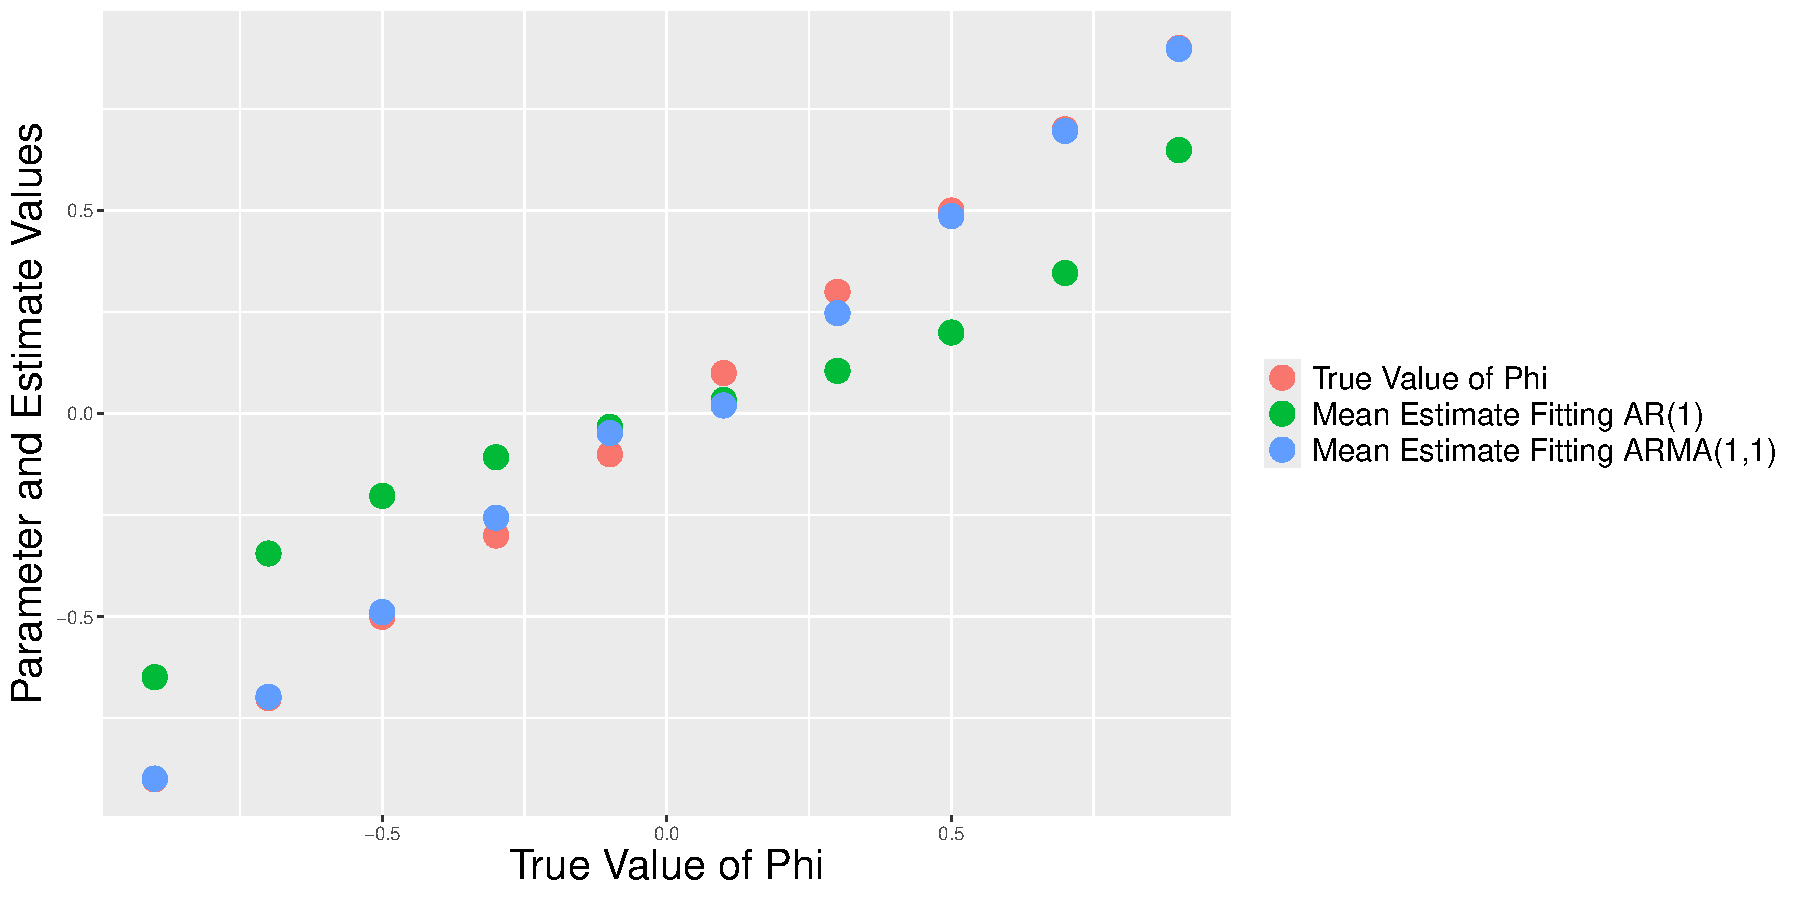
\includegraphics[width=\linewidth]{../figures/ar_bias.pdf}
    \caption{Aggregated estimates for AR. An interactive version of this
    figure is available
    \href{run:../figures/phi_3d_plot.html}{here}.}
    \label{fig:ar_bias}
\end{figure}

It is also worth noting that it is not currently possible to tease apart the two sources 
of noise. This is only possible if there are multiple noisy observations of each time series element.
We now proceed to examine the efficacy with which the methodology of fitting ARMA-Noise Models--here generalized for varying sample sizes--does just that.





\subsection{Empirical Confidence of ARMA-Noise Models}
Before applying the REMARCS algorithm in its entirety to simulated data, it would
be prudent to verify that generalizing ARMA-Noise Models to allow for 
varying sample sizes still produces valid estimates.

We begin with simulations of an ARMA(1,1)-Noise Model:
 $$y_{ti} = u_t + {\varepsilon}_{ti}, \qquad u_t - \phi u_{t-1} = \eta_t + \theta \eta_{t-1} $$ 
 
 
 $$\quad t = 1,...,T \quad i = 1,...,n_t \quad n_t \overset{i.i.d.}{\sim} \text{Poi}(\lambda) + 1 $$
 
Differing values of $\phi$ and $\theta$ were combined with fixed parameters $\sigma_\varepsilon^2 = \armanconfveps$, $\sigma_\eta^2 = \armanconfveta$, and $\lambda = \armanconflambda$.
For each value-pair $(\phi,\theta)$, $\armanconfsims$ simulations are generated and used to estimate
parameter values. Covariance matrices are estimated and used to calculate empirical confidence levels with $\alpha = \armanconfalpha$ 
(see Figure \ref{fig:e_conf_l}).

COMMENT on use of method of moments estimator for wong

 defined by $w_t = \bar{\yy}_{t\cdot}$, with MA parameter $\theta_b$ and innovation variance $\sigma_b^2$, 
 produces time series estimates with normalized covariance close to $\Sigma_{\phi,\theta_b}$. For each set 
 of parameters, we calculate the true values of $\theta_b$ and $\sigma_b^2$.  We then fit $(\hat{\phi},\hat{\theta}_b)$ 
 with $\bar{\mathbf{w}}$ and construct confidence regions centered around those estimates, counting the rates at 
 which these confidence regions capture the true parameter values. These empirical confidences are displayed in 
 Figure \ref{fig:e_conf_l}. 

CHECK THAT DELTA METHOD IS TAKING DERIVATIVES W.R.T. VEPS NOT VARA



\begin{figure}[htbp]
\centering
    \begin{subfigure}{0.45\linewidth}
        \centering
        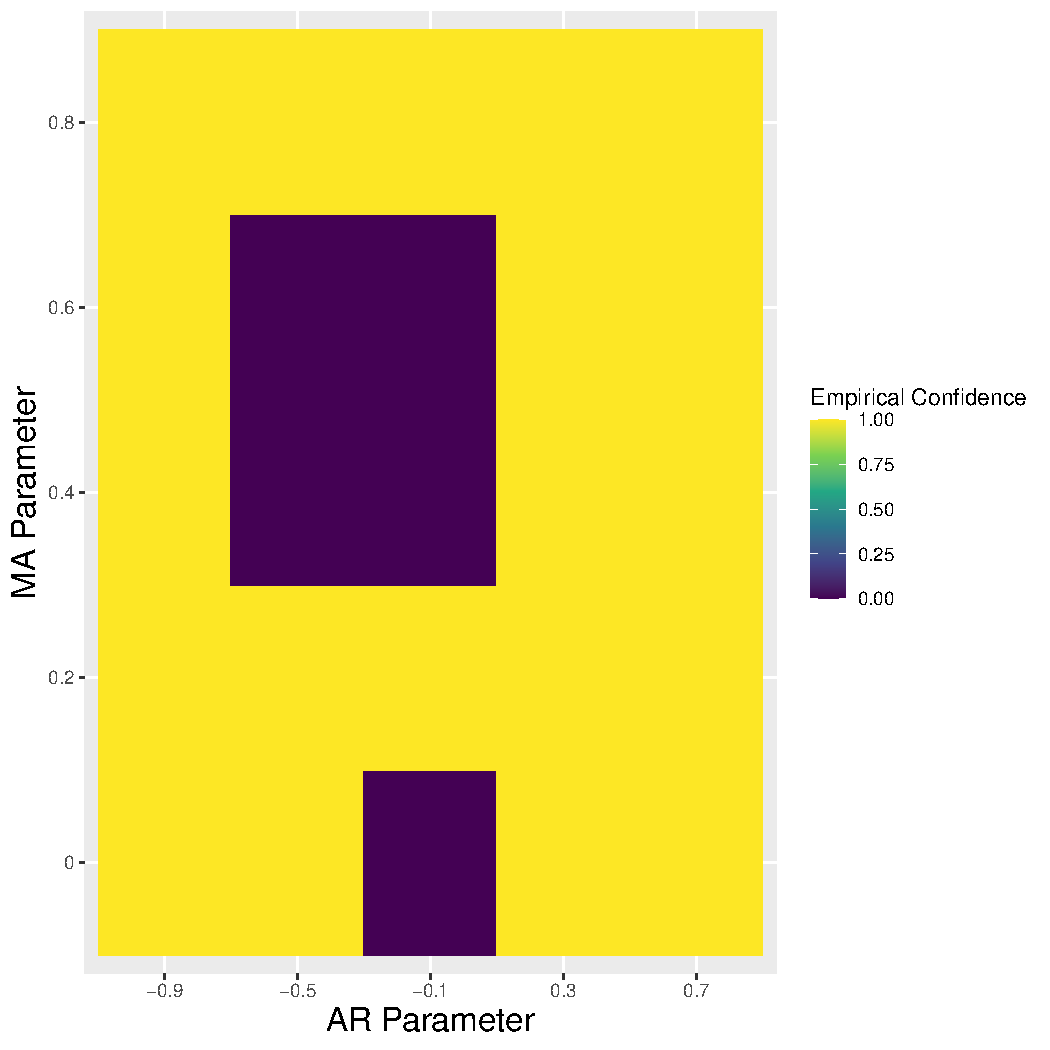
\includegraphics[width=\linewidth]{../figures/e_conf_l_3_2.pdf}
        \subcaption{$T = \armanconfTleft$}
    \end{subfigure}
    \hfill
    \begin{subfigure}{0.45\linewidth}
        \centering
        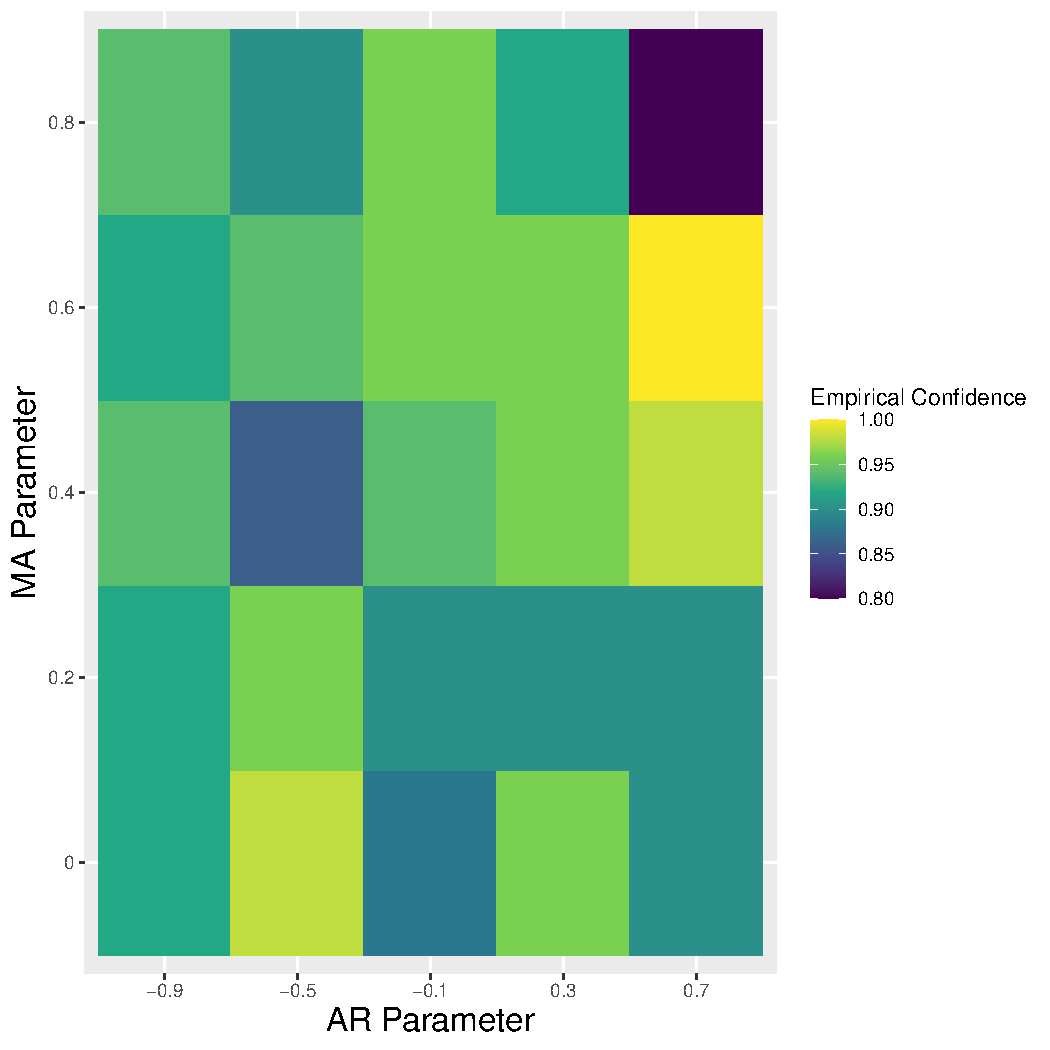
\includegraphics[width=\linewidth]{../figures/e_conf_l_4_2.pdf}
        \subcaption{$T = \armanconfTright$}
        
    \end{subfigure}
    \caption{Rates at which point estimates for $\tau_l$ fall within confidence regions based on sample estimates}
    \label{fig:e_conf_l}
\end{figure}




We can see performance dipped for parameter combinations $(\phi,\theta)$ close to the $\phi + \theta = 0$ line for time series of length $T = \armanconfTleft$. However, we can see that performance improved for $T=\armanconfTright$, suggesting that parameter estimates for ARMA(1,1) processes that resemble white noise take longer to converge to their asymptotic distributions.
\subsection{Instability of EM Algorithm}

To highlight the necessity for a different approach to fitting latent parameters,
we test the stability of time series parameters using an EM algorithm. We define our model
to be as follows:

$$ y_{ti} = \mathbf{x}_{ti} \beta + u_t + \varepsilon_{ti}, \qquad t = 1,...,T $$
$$i = 1,...,n_t \qquad n_t \overset{i.i.d.}{\sim} \text{Poi}(\lambda) + 1 $$

Here, $\uu$ is defined to be an AR(1) process with innovation variance $\sigma_\eta^2 = \areveta$. 
Other fixed parameters include $\sigma_\varepsilon^2 = \areveps$, $T = \areT$, and $\beta = c(\areint,\areslope,\arecov)$.
For varying values of $\phi$, $\aresims$ realizations of the model were simulated,
and for each simulation, \emph{true values for all parameters} were used to 
estimate $\hat{\uu} = \Sigma_\uu X_t' \Sigma_\yy^{-1}(\yy - X_f \beta)$. That estimate
was then used to fit an AR(1) model, updating $\hat{\phi}$ just as would be done
via the EM algorithm (in the unlikely event all parameters were unwittingly estimated perfectly).
Results are displayed in Table \ref{tab:are_stability}.

\input{../figures/are_tab.txt}

It is immediately apparent that even in the event of perfect parameter estimation,
the resulting time series estimate $\hat{\uu}$ is not an AR(1) process and more 
importantly will yield biased estimates for time series parameters if treated as one.
Having demonstrated the need for the REMARCS Algorithm, we now turn to evaluating 
its efficacy.

\subsection{Empirical Confidence of REMARCS algorithm}

Now 

In order to assess the efficacy of this method, $ \simsfearma $ simulations were conducted with 
fixed parameters $\beta = (\intfearma,\slopefearma,\xfearma)$, $\sigma_\eta^2 = \vetafearma$, 
$ \sigma_\varepsilon^2 = \vepsfearma$, and varying combinations of ARMA parameters $(\phi,\theta)$. 

In Figure \ref{fig:conf_heatmap}, we can see the proportion of simulations that yielded 
confidence regions successfully capturing $\beta$ (left) and $(\phi,\theta,\sigma_\eta^2)$ (right). 
One observation we can make is that, similarly to the ARMA-Noise simulations, convergence
to asymptotic distributions is slower for parameter combinations close to the line $\phi + \theta = 0$. 
This under-performance is mitigated as $T$ grows, indicating that time series more closely resembling white noise 
will require larger values of $T$ for accurate estimation. 

EXCLUDE VETA FROM CONFIDENCE REGIONS FOR RIGHT PANEL

\begin{figure}[htbp]
    \centering
    \begin{subfigure}{0.48\textwidth}
        \centering
        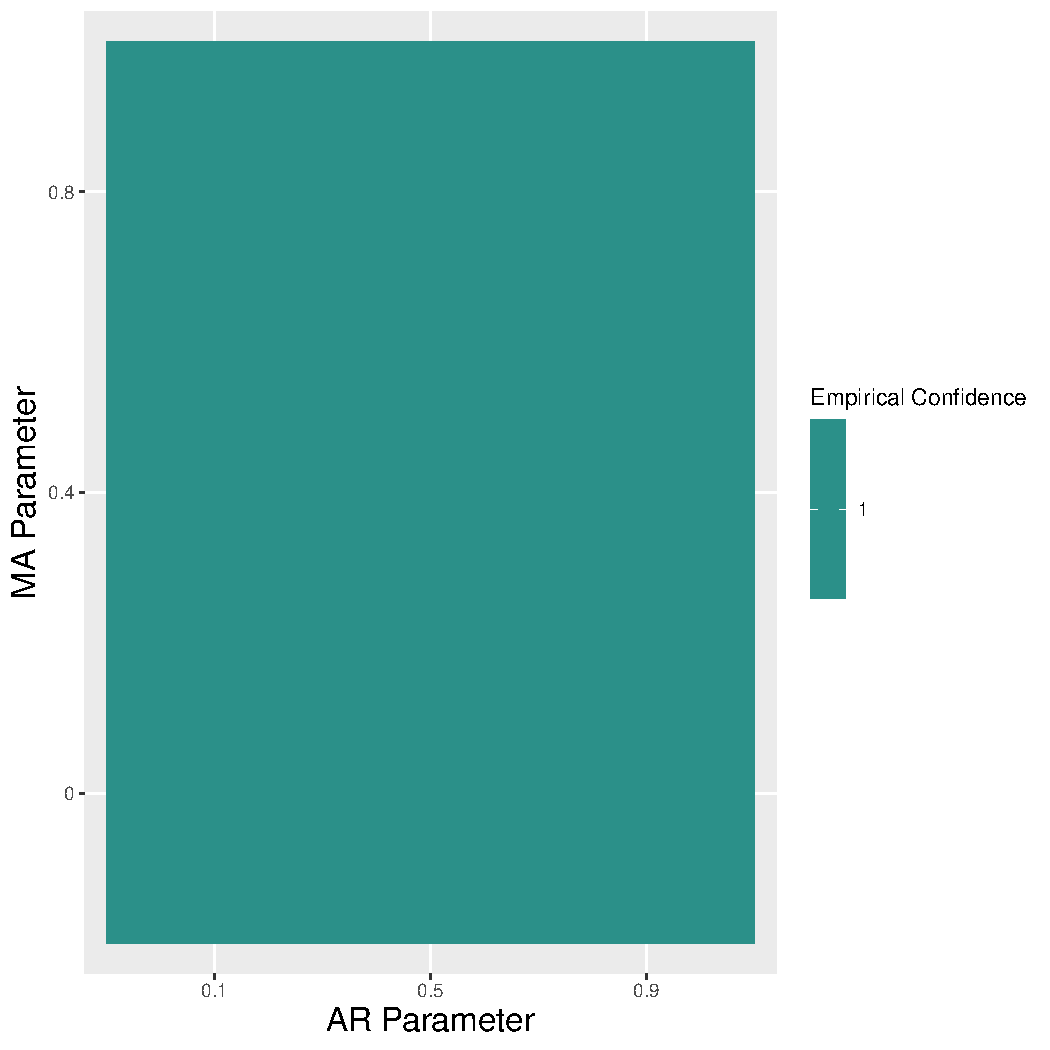
\includegraphics[width=\linewidth]{../figures/l1_conf.pdf}
        \caption{Fixed Effect Parameter Estimation}
        \label{fig:sub1}
    \end{subfigure}
    \hfill
    \begin{subfigure}{0.48\textwidth}
        \centering
        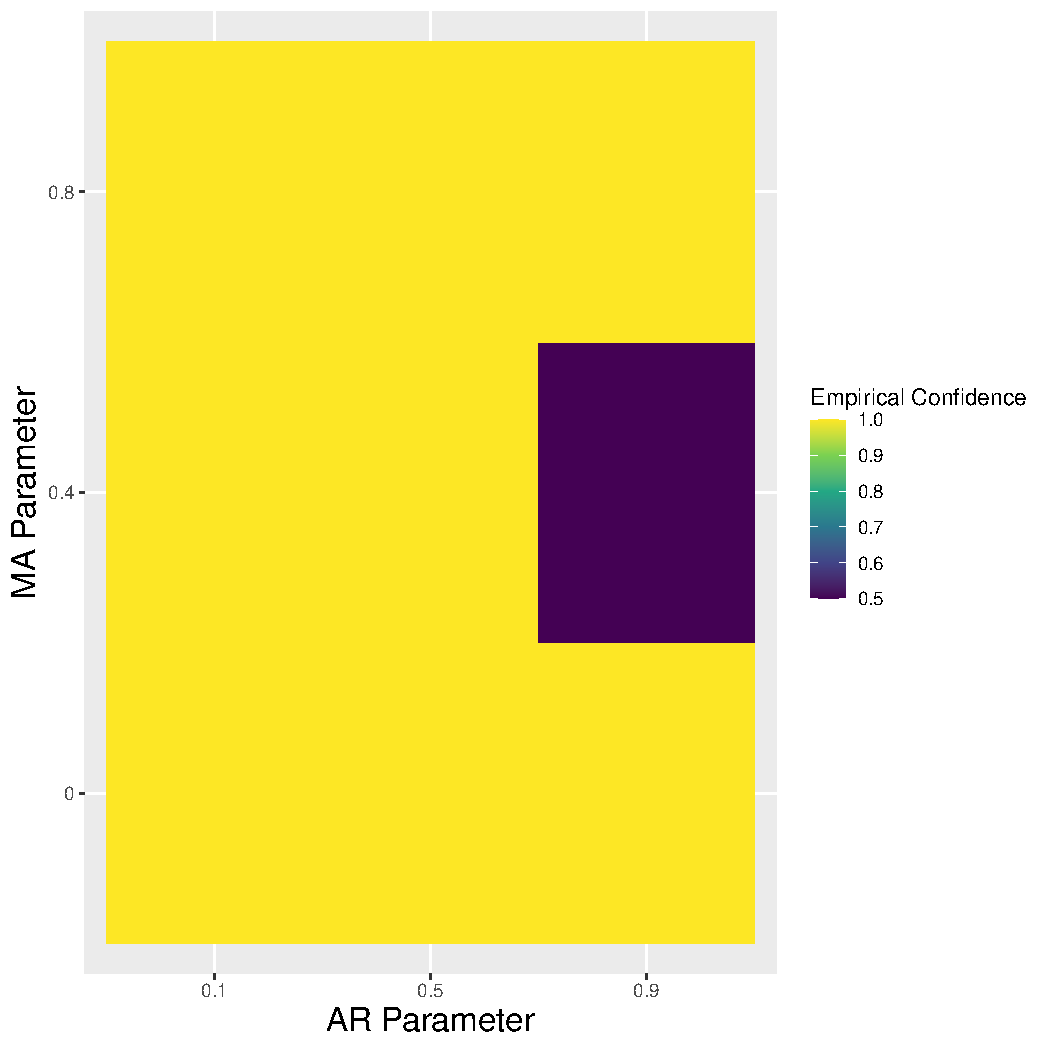
\includegraphics[width=\linewidth]{../figures/l2_conf.pdf}
        \caption{Time Series Parameter Estimation}
        \label{fig:sub2}
    \end{subfigure}
    \caption{Empirical confidences with which model parameters fall within confidence regions generated after model convergence}
    \label{fig:conf_heatmap}
\end{figure}
\subsection{Empirical Confidence of Model Selection}


Now that we've seen some aggregate results displaying the efficacy of this method under different parameters,
we aim to evaluate the algorithm's ability to identify when model restriction is necessary.
% \subsection{Case: $\uu$ and $\mathbf{w}$ are ARMA(1,1)}

We start with the case in which $\uu$ is an AR(1) process. We simulate REMARCS models with 
such a latent time series, tracking the rate at which the algorithm yields an insignificant estimate for $\theta$.
Fixed parameters include $T = \uarT$, $\sigma_\eta^2 = \uarveta$, $\sigma_\varepsilon^2 = \uarveps$, $\lambda = \uarlambda$, 
$\beta = (\uarint,\uarslope,\uarcov)$. For each value of $\phi$, $\uarsims$ realizations were simulated
and the REMARCS algorithm applied. Displayed below are the rates at which parameter estimates for 
$\theta$ were deemed insignificant.

\input{../figures/uar_tab.txt}


We now proceed to the case in which $\uu$ is an MA(1) process. We simulate REMARCS models with 
such a latent time series, tracking the rate at which the algorithm yields an insignificant estimate for $\phi$.
Fixed parameters include $T = \uarT$, $\sigma_\eta^2 = \uarveta$, $\sigma_\varepsilon^2 = \uarveps$, $\lambda = \uarlambda$, 
$\beta = (\uarint,\uarslope,\uarcov)$. For each value of $\theta$, $\umasims$ realizations were simulated
and the REMARCS algorithm applied. Displayed below are the rates at which parameter estimates for 
$\phi$ were deemed insignificant.

\input{../figures/uma_tab.txt}

From these results we can see that the algorithm effectively identifies when model restriction is necessary.







\subsection{Method Comparison}

We begin with a realization of a REMARCS model (Figure \ref{fig:sample_are}) with parameters detailed in Table \ref{tab:sample_are}. 
The moving average parameter $\theta$ has been set to zero so the model is consistent with the ARE model detailed by Modugno et al.

Our best attempt to recreate the ARE algorithm encounters convergence problems, likely due to inappropriately
fitting time series estimates with an AR(1) time series.



\begin{table}[htbp]
    \centering
    \begin{tabular}{c|c|c|c|c|c|c|c}
        Parameter   & Intercept     & Slope     &  Dummy Indicator     & $\sigma_\varepsilon^2$    & $\phi$    & $\theta$  & $\sigma_\eta^2$\\
        \hline 
        Value       & $\intrcpt$    & $\slope$      & $\covind$     & $\vareps$                 & $\ar$     & $\ma$     & $\vareta$
    \end{tabular}
    \caption{Parameter values for simulated ARE model}
    \label{tab:sample_are}
\end{table}

\begin{figure}[htbp]
    \centering
    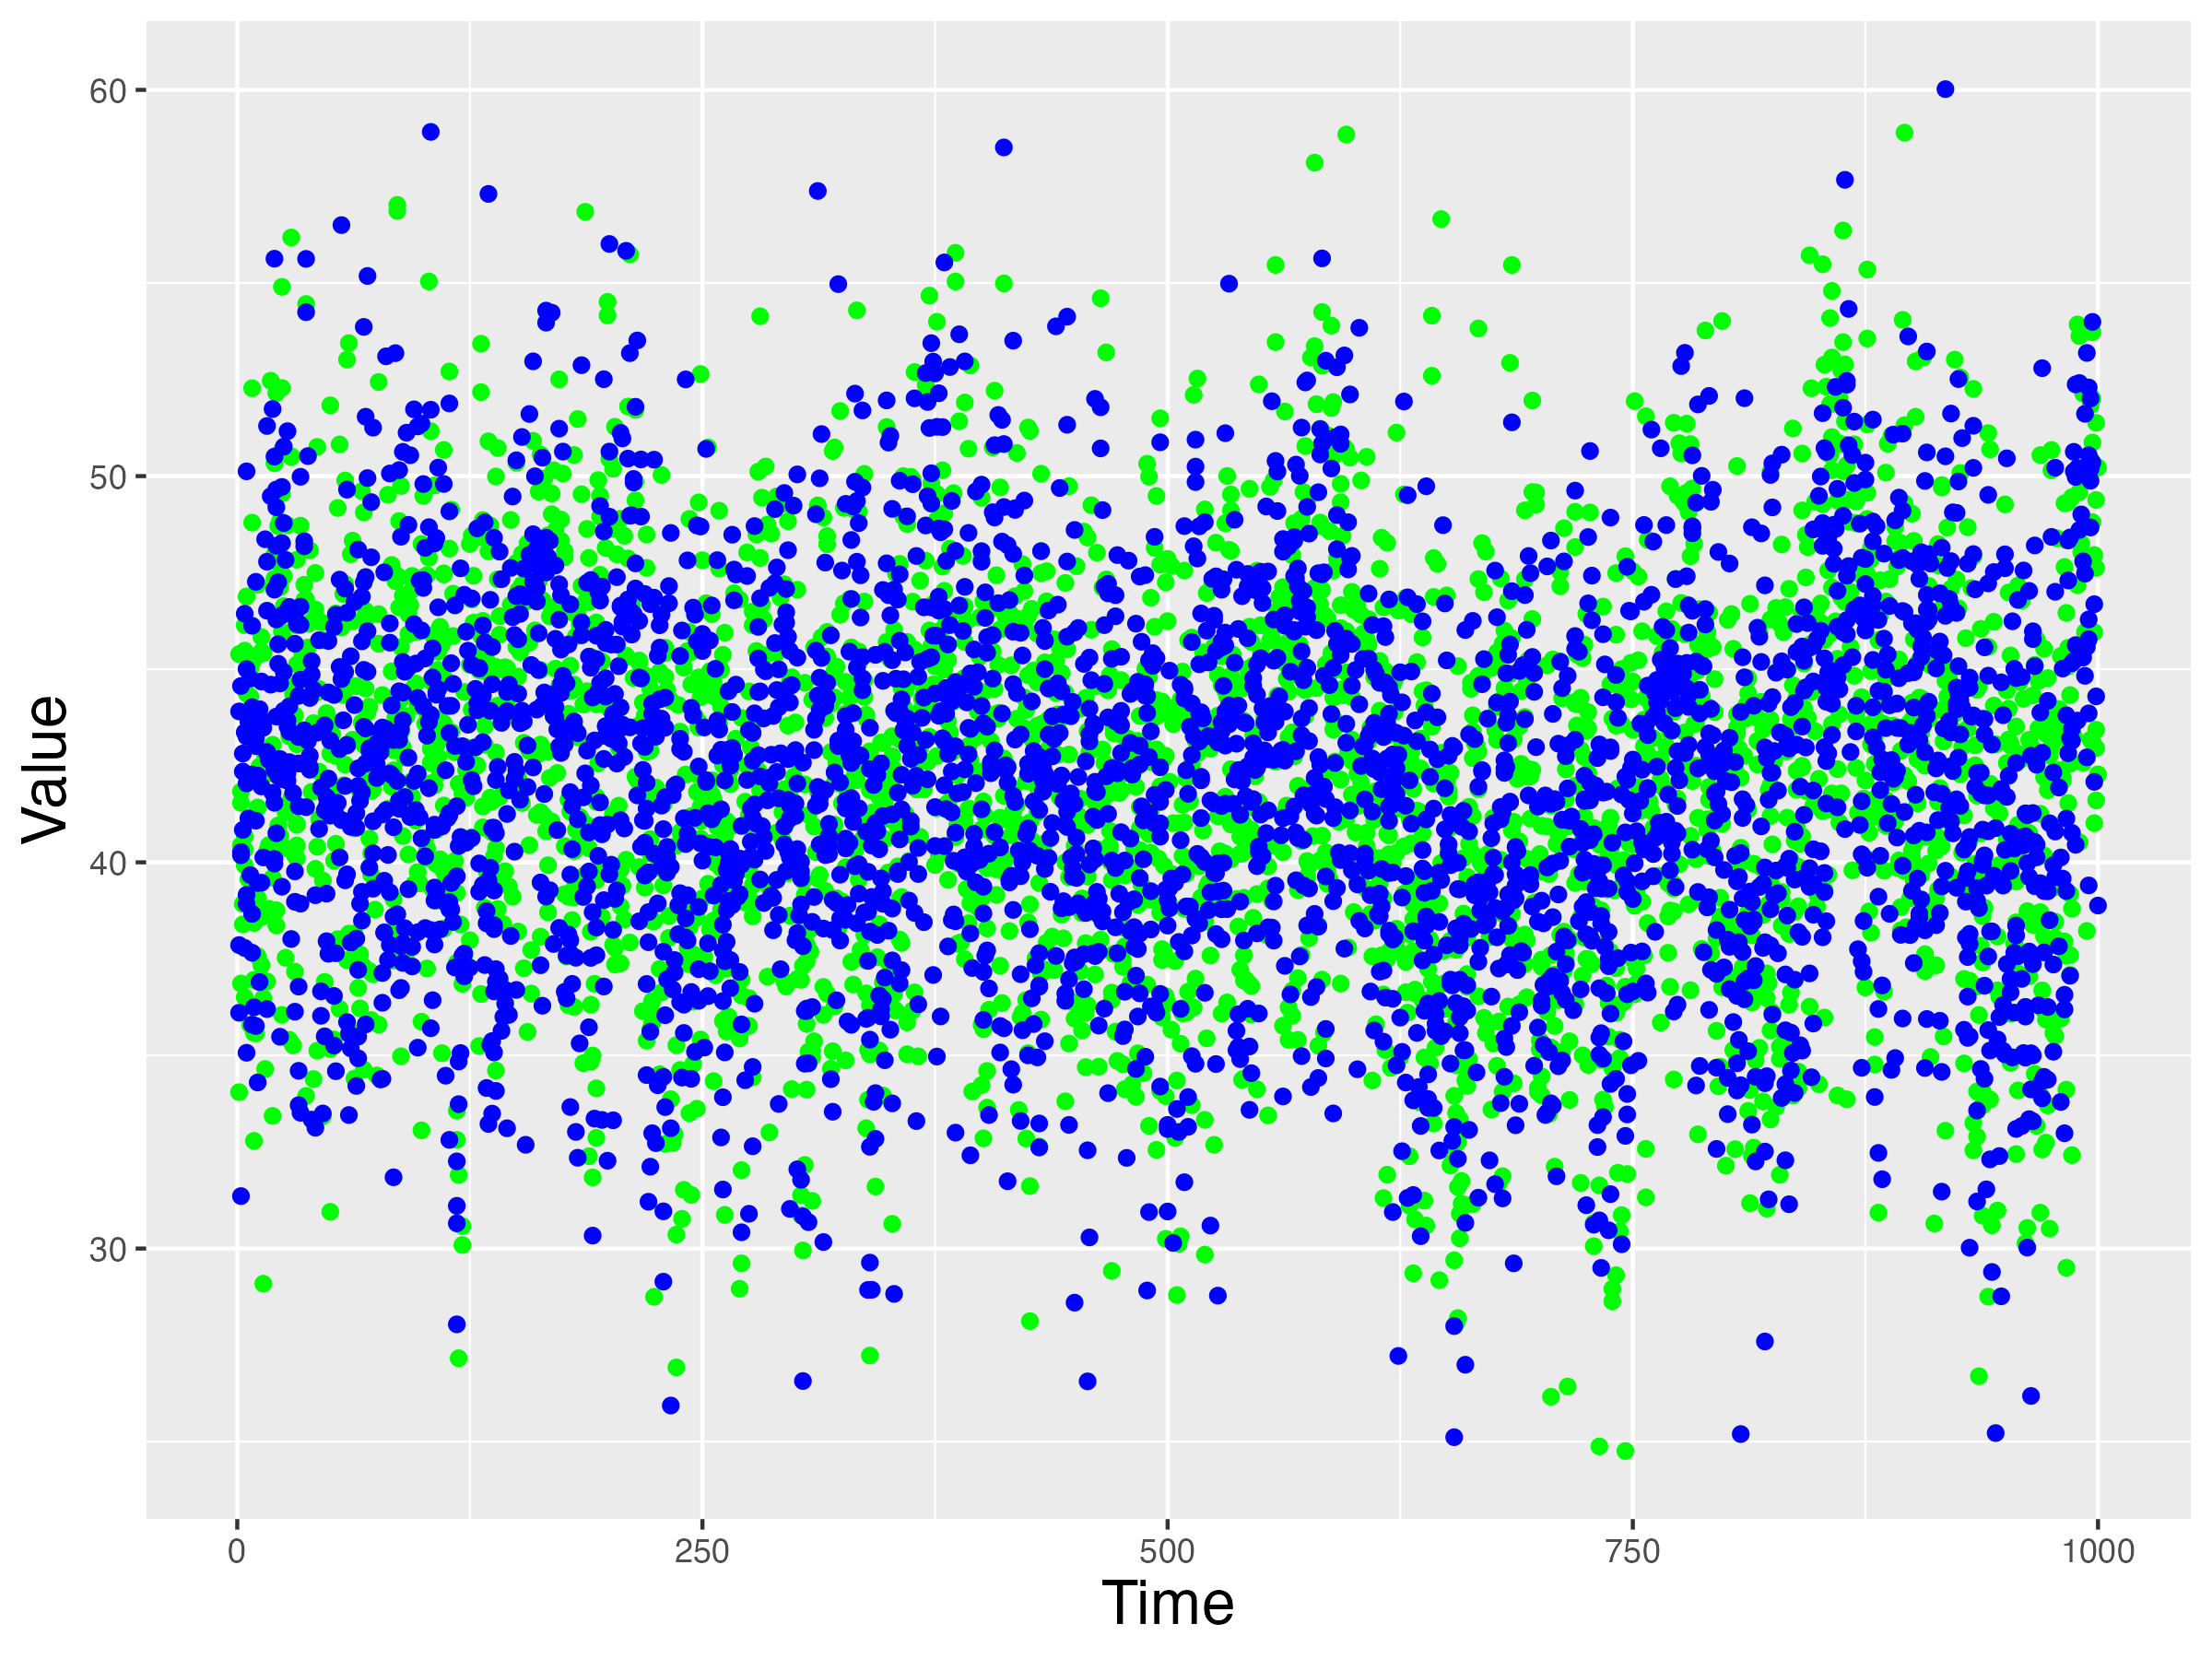
\includegraphics[width=0.6\linewidth]{../figures/are.png}
    \caption{Realization of ARE model with parameters defined in Table \ref{tab:sample_are}}
    \label{fig:sample_are}
\end{figure}

% \subsection{Simulations}

We now compare the performance of the REMARCS algorithm with those of 
the ARE model and fitting a time series with covariates.


We consider fitting this model by aggregating the data at each time point 
and treating the averages as a time series with covariates. $\sims$ 
simulations were generated and fit with each method.



Some sample rows of simulated data are provided below:


\input{../figures/arma_cov_head.txt}

After aggregating at each time step, we obtain the following condensed dataset, from which a time series with 
covariates is then fit:

\input{../figures/arma_cov_head_daily.txt}


If we then fit a time series with covariates to the condensed dataset, we obtain results with empirical means 
displayed in the table below. The ``Significance Frequency" column displays the fraction of the hundred 
simulations in which the corresponding parameter estimate was statistically significant at the $\alpha = .05$ 
level.


\input{../figures/arma_cov_df.txt}


Note that entries of the \textit{x} column, while displaying some variability, are fairly close to $0.5$. 

ADD STANDARD ERRORS!!! CHANGE SIGNIFICANCE TO EMPIRICAL CONFIDENCE
DOUBLE CHECK SIGMAO FUNCTION, VAREPS OR VARA
% Note that the effect of the dummy indicator variable is deemed significant only
%  $\covconf\%$ of the time. This example highlights the shortcomings of fitting a time series with covariates.
%   Also of note is how skewed the sample mean of $\hat{\theta}$ is. This is because what we are in fact estimating is 
%   $\theta_b$, the MA parameter of $\mathbf{w}$



\begin{itemize}
    \item SIMULATE FIXED/MIXED EFFECT REMARCS DATA
    \item FIT WITH FE/ME MODEL
    \item FIT WITH TS WITH COVARIATES
    \item MODUGNO INSTABILITY
    \item FIT WITH REMARCS
    \item HEATMAPS
    \item MODEL SELECTION
\end{itemize}

RCSFIXED CANT CURRENTLY HANDLE MISSING VALUES

Now that our algorithm has demonstrated promising results on simulated data, we observe how it performs on real RCS survey data.